\chapter{Event Generation and Reconstruction}\label{chap:MCGenReco}


The events used for this measurement were reconstructed from data acquired by the CMS detector in the case of the data and generated using Monte Carlo generators PYTHIA and HERWIG in the case of the generated data.

\section{Brief Introduction to Monte Carlo Event Generators}\label{secMCGen}

Monte Carlo (MC) event generators are tools used by both experimental and theoretical physicists to simulate different physical processes in order to make predictions and prepare future experiments. The main tasks of such generators are to calculate matrix elements of the relevant hard processes but they must also describe parton showering, hadronization and underlying event. MC can be utilized to extrapolate data measurements beyond the acceptance of the detector or in the case of this thesis it is used in the unfolding process to correct the data for detector efficiency and resolution.


MC generators provide an ensemble of generated events that simulate the physics process in question. Each individual generator implements a slightly different scheme in order to approximate the necessary calculations for the factorization and renormalization scales relevant to a process. These variations mean that the choice of MC generator will have a slight effect on the generated distributions. For this reason, in the analysis described herein we compared results from 2 different generators: PYTHIA and HERWIG.



All event generators break the calculations into separate parts as depicted by the different colored objects in Figure ~\ref{fig:MCeventpretty}  


\begin{figure}[htb]
\centering
\includegraphics[width=1.0\textwidth]{visuals/MCeventpretty.png}
\caption{A pictorial representation of the way the MC generators simulate hadron-hadron collisions~\cite{Hoche:2014rga}.}
\label{fig:MCeventpretty}
\end{figure}





PYTHIA ~\cite{Sjostrand:2006za} is a very commonly used general purpose event generator which uses the parton shower approach for higher order corrections to the hard scattering matrix element.

HERWIG  ~\cite{herwigpp} is another commonly used event generator, incredibly similar to PYTHIA, differing mainly in hadronization and parton showering behaviors.


\section{Event Reconstruction with Particle Flow}\label{sec:PFReco}


The data from proton-proton collisions at LHC are detected by the CMS experiment and then the Particle Flow (PF) event reconstruction ~\cite{Sirunyan:2017ulk} is applied to these raw detector outputs in order to construct "particle flow objects" that contain information from multiple CMS detector subsystems and constitute a global event description. More details about the CMS apparatus can be found in Chapter~\ref{chap:CMS}. The particle flow objects are given defined object categories based on which subsystems they are measured in. This requires the use of a "link algorithm" which combines subdetector information together into a single object ~\cite{Sirunyan:2017ulk}. For example, one can see that the solid, light blue, line in Figure ~\ref{fig:cmsPF} corresponds to a muon PF object as it left hits in the tracker then traversed all of the calorimeters only to deposit its energy in the muon chambers.


\begin{figure}[htb]
\centering
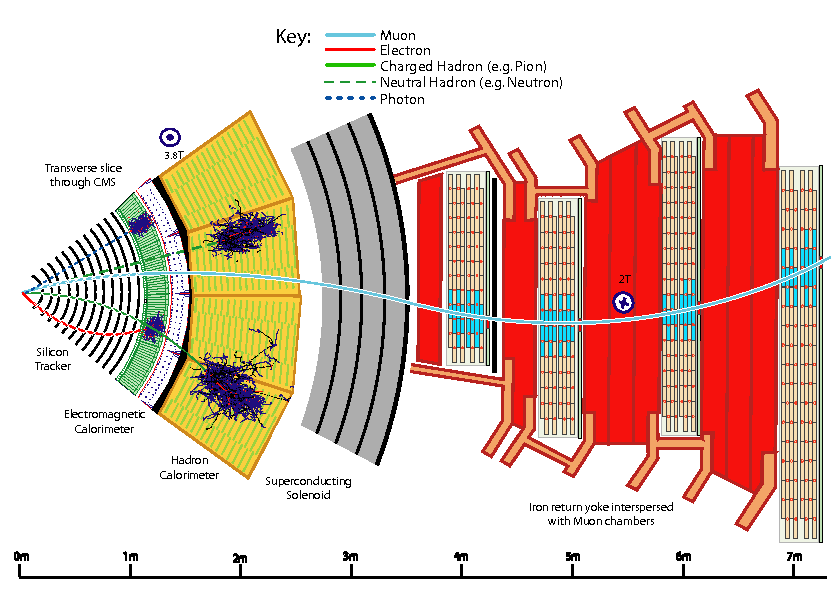
\includegraphics[width=1.0\textwidth]{Chapter-1/cmsPflow.png}
\caption{A pictorial representation of the way the Particle Flow algorithm determines which objects correspond to which particles based on an optimal combination of sub-detector information ~\cite{Sirunyan:2017ulk}.}
\label{fig:cmsPF}
\end{figure}


 PF aims to reconstruct and identify each individual particle in an event, with an optimized combination of all subdetector information. In doing so PF characterizes the particles into 5 types: photon, electron, muon, charged hadron, neutral hadron. The type determines which sub-detector information will be combined to determine the energy and direction of that particle. Photons (\eg coming from electron bremsstrahlung) are identified as ECAL energy clusters that are not linked to the extrapolation of any charged particle trajectory to the ECAL. Electrons (\eg coming from photon conversions in the tracker material or from semileptonic decays of hadrons) are identified as a primary charged particle track and potentially many ECAL energy clusters corresponding to this track extrapolation to the ECAL and to any bremsstrahlung photons emitted along the way within the tracker. Muons (\eg from  hadron semileptonic decays) are identified as tracks in the central tracker consistent with either a track or several hits in the muon system, and associated with calorimeter deposits compatible with the muon hypothesis. Charged hadrons are identified as charged particle tracks neither identified as electrons, nor as muons. Finally, neutral hadrons are identified as HCAL energy clusters not linked to any charged hadron trajectory, or as a combined ECAL and HCAL energy excess with respect to the expected charged hadron energy deposit.

The ECAL is used to obtain the energy of photons. The energy of electrons is more complex, determined from a combination of the track momentum at the main interaction vertex, the corresponding ECAL cluster energy, and the energy sum of all bremsstrahlung photons originating from the track. The energy of muons is obtained from the corresponding track momentum. The energy of charged hadrons is determined from a combination of the track momentum and the corresponding ECAL and HCAL energies, corrected for zero-suppression effects and for the response function of the calorimeters to hadronic showers. Finally, the energy of neutral hadrons is obtained from the corresponding corrected ECAL and HCAL energies.

After particle flow is used to determine the particle's type, the particle flow objects which are not categorized as muons, electrons and isolated photons are then described as hadrons and are clustered into "jets". An example PF jet with 5 constituent PF objects is depicted in Figure~\ref{fig:cmsPFjet}.

\begin{figure}[htb]
\centering
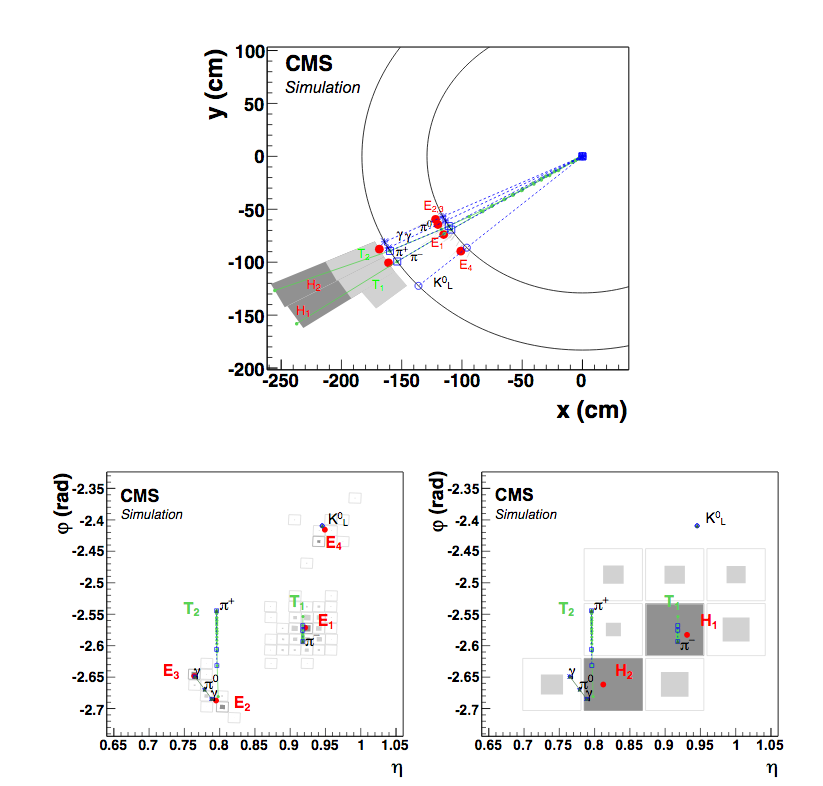
\includegraphics[width=1.0\textwidth]{Chapter-1/cmsPflowjet.png}
\caption{A pictorial representation of the way the Particle Flow objects are clustered into jets ~\cite{Sirunyan:2017ulk}. The top image shows a jet composed of 5 PF candidates in the x,y plane and the concentric circles describe the surfaces of the ECAL and HCAL detectors respectively. The lower left image is the PF candidates as measured by the ECAL and the image on the lower right shows the same for the HCAL surface. The dotted lines represent generated particles and the solid boxes represent energy deposits in the detector. }
\label{fig:cmsPFjet}
\end{figure}

For each event, hadronic jets are clustered from these reconstructed particles using the infrared and collinear safe anti-\kt algorithm~\cite{Cacciari:2008gp, Cacciari:2011ma} with a distance parameter of 0.4. Jet momentum is determined as the vectorial sum of all particle momenta in the jet, and is found from simulation to be, on average, within 5 to 10\% of the true momentum over the whole \pt spectrum and detector acceptance. Additional proton-proton interactions within the same or nearby bunch crossings (pileup) can contribute additional tracks and calorimetric energy depositions to the jet momentum. 

The pileup per particle identification (PUPPI) algorithm~\cite{Bertolini:2014bba} is used to mitigate the effect of pileup at the reconstructed particle level, making use of local shape information, event pileup properties and tracking information. Charged particles identified to be originating from pileup vertices are discarded. For each neutral particle, a local shape variable is computed using the surrounding charged particles compatible with the primary vertex within the tracker acceptance ($|\eta| < 2.5$), and using both charged and neutral particles in the region outside of the tracker coverage. The momenta of the neutral particles are then rescaled according to their probability to originate from the primary interaction vertex deduced from the local shape variable, superseding the need for jet-based pileup corrections~\cite{CMS-PAS-JME-16-003}. 


%To mitigate this effect, charged particles identified to be originating from pileup vertices are discarded and an offset correction is applied to correct for remaining contributions. Jet energy corrections are derived from simulation to bring measured response of jets to that of particle level jets on an average. In situ measurements of the momentum balance in dijet, $\text{photon} + \text{jet}$, $\PZ + \text{jet}$, and multijet events are used to account for any residual differences in jet energy scale in data and simulation~\cite{Khachatryan:2016kdb}. The jet energy resolution amounts typically to 15\% at 10\GeV, 8\% at 100\GeV, and 4\% at 1\TeV. Additional selection criteria are applied to each jet to remove jets potentially dominated by anomalous contributions from various subdetector components or reconstruction failures. 


